\section*{Execution flow}\label{execution_flow}
When it comes to understanding the actual flow of execution in a MapReduce cluster, two parameters need to be discussed:
\begin{itemize}
    \item \textit{The number of splits \textbf{M} (Map input)}\\
    This value determinates how many portions the input data will be divided into; this value should be set accordingly to have each portion between 16 and 64 Mb in size.
    \item \textit{The number of intermediate key partitions \textbf{R} (Reduce input)}\\
    The intermediate key space is partitioned into R pieces using a partitioning function (e.g. \textit{hash(key) mod R} \cite{google_mapreduce}), distributing the Reduce invocations. R is usually a small multiple of the number of cluster machines that will be used.
\end{itemize}
The partitioning function, M and R can be set by the user. Typically, MapReduce operations performed at Google have M=200000 and R=5000 with 2000 machines \cite{google_mapreduce}.

The Master, acting as coordinator and intermediary among the Worker nodes, mainly keeps two data structures in memory:
\begin{itemize}
    \item \textbf{Tasks' state}\\
    For every Map task and every Reduce task (for a total number of M + R), the Master keeps track of the current state, that can be either idle, in progress or completed.
    \item \textbf{Intermediate results location}\\
    The master stores the locations and sizes of the R intermediate file regions produced by the map task in order to communicate said data to the Reduce Workers that are in the "in progress" state.
\end{itemize}

\begin{figure}[!ht]
    \centering
    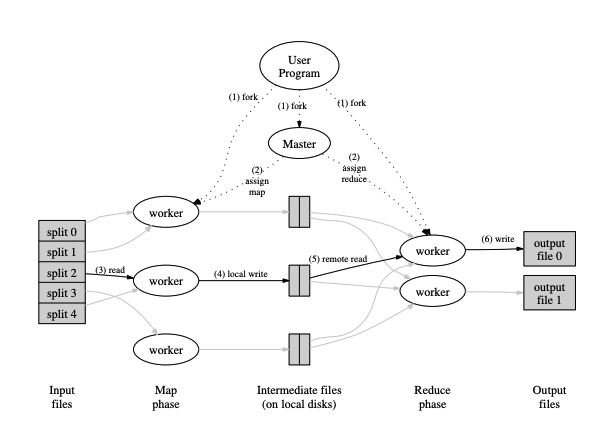
\includegraphics[scale=0.75]{document/appendix/appendix_1/images/mapreduce_execution_flow.png}
    \caption{MapReduce execution flow \cite{google_mapreduce}}
    \label{fig:mapreduce_execution_flow}
\end{figure}

\textit{Figure \ref{fig:mapreduce_execution_flow}} shows an example of execution flow (the enumeration in the following list corresponds to the numeric labels displayed in the figure) with M=5, R=2 and 6 machines (the R parameter has not an optimal value, but this is done only for explanatory reasons):
\begin{enumerate}
    \item The MapReduce library on the User program side splits the input accordingly to the M parameter and starts many copies of the program on the cluster's machines. One of the machines acts as the Master and the others as Workers (\textit{section \ref{map_reduce_architecture}}). The Map and Reduce functions' code is propagated to the machines and the User Program waits to be notified by the Master after the completion of the MapReduce tasks.
    \item The Master assigns the total M + R tasks to the Workers, be it a Map task or a Reduce task.
    \item A Worker that executes a Map task reads the corresponding input piece among the M parts. The key/value pairs are processed through the User-defined Map function and the intermediate results are buffered in memory.
    \item Periodically, the buffered intermediate results are written on the local disk. Said results are partitioned locally in R regions following the partitioning function. After that, the Worker communicates the location of such results to the Master which, in turn, forwards this information to the Reduce Workers.
    \item When a Worker is notified about the availability of new results, it reads them (using the location previously provided) from the correct Workers and, once it has all the data for its region, it sorts such data using the intermediate key, grouping together data that belongs to the same key. If the intermediate data is too large to fit in memory, the sorting is done using the disk.
    \item The Worker iterates over the data and, for each key, performs the Reduce function provided by the User. This produces a file containing all the Reduce results for the region handled by the Worker.
    \item After all the Map and Reduce tasks are completed, the User program is notified, and it can resume its execution.
\end{enumerate}

The final output of the R files can then be accessed as it is, combined into a single source, or used as input for a new MapReduce execution.